\chapter{Конструкторская часть}

В данном разделе будут указаны требования к программному обеспечению и представлены схемы алгоритмов сортировки выбором, бусинами и блочной сортировки.

\section{Требования к программе}

К программе представлен ряд требований:

\begin{itemize}
	\item на вход подается массив целых чисел;
	\item на выходе - отсортированный массив, поданный на вход и временные замеры алгоритмов.
\end{itemize}

\section{Разработка алгоритмов}

На рисунках \ref{img:selection_sort}, \ref{img:bead_sort}, \ref{img:bucket_sort} представлены схемы алгоритмов сортировки выбором, бусинами и блочной сортировки.

\begin{figure}[H]
	\begin{center}
		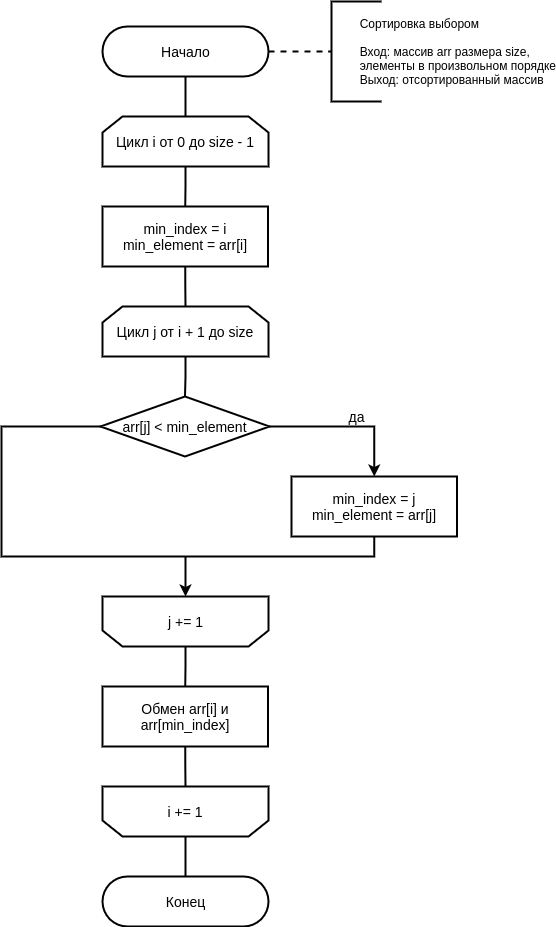
\includegraphics[scale=0.5]{img/selection_sort.png}
	\end{center}
	\captionsetup{justification=centering}
	\caption{Схема алгоритма сортировки выбором}
	\label{img:selection_sort}
\end{figure}

\begin{figure}[H]
	\begin{center}
		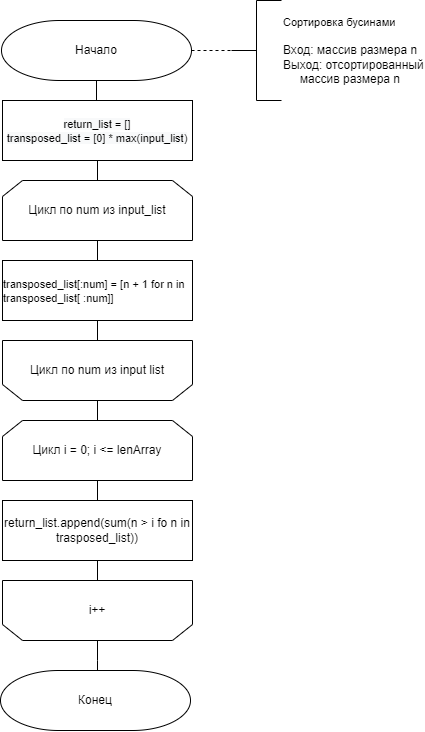
\includegraphics[scale=0.5]{img/bead_sort.png}
	\end{center}
	\captionsetup{justification=centering}
	\caption{Схема алгоритма сортировки бусинами}
	\label{img:bead_sort}
\end{figure}

\newpage

\begin{figure}[H]
	\begin{center}
		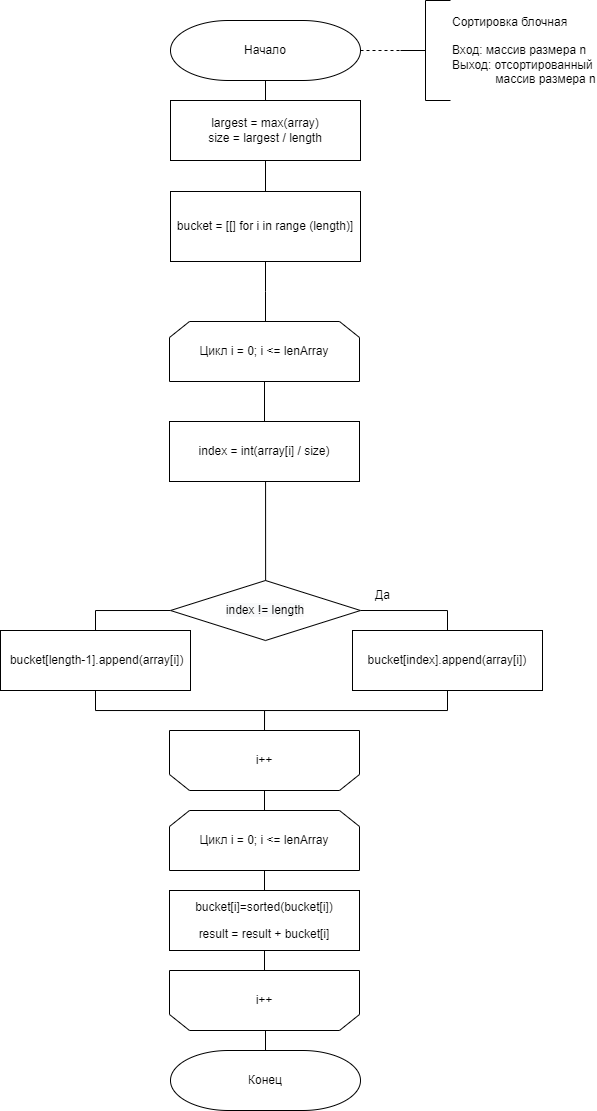
\includegraphics[scale=0.5]{img/bucket_sort.png}
	\end{center}
	\captionsetup{justification=centering}
	\caption{Схема алгоритма блочной сортировки}
	\label{img:bucket_sort}
\end{figure}

\section{Модель вычислений для оценки трудоёмкости алгоритмов}

Для определения трудоемкости алгоритмов необходимо ввести модель вычислений:

\begin{enumerate}
	\item операции из списка (\ref{for:operations}) имеют трудоемкость равную 1;
	\begin{equation}
		\label{for:operations}
		+, -, /, *, \%, =, +=, -=, *=, /=, \%=, ==, !=, <, >, <=, >=, []
	\end{equation}
	\item трудоемкость оператора выбора \code{if условие then A else B} рассчитывается, как (\ref{for:if});
	\begin{equation}
		\label{for:if}
		f_{if} = f_{\text{условия}} +
		\begin{cases}
			f_A, & \text{если условие выполняется,}\\
			f_B, & \text{иначе.}
		\end{cases}
	\end{equation}
	\item трудоемкость цикла рассчитывается, как (\ref{for:cycle});
	\begin{equation}
		\label{for:cycle}
		f_{for} = f_{\text{инициализации}} + f_{\text{сравнения}} + N(f_{\text{тела}} + f_{\text{инкремент}} + f_{\text{сравнения}})
	\end{equation}
	\item трудоемкость вызова функции равна 0.
\end{enumerate}

\section{Трудоёмкость алгоритмов}

Проведем сравнительный анализ реализованных алгоритмов по трудоемкости.

\subsection{Алгоритм сортировки выбором}

Трудоемкость в лучшем случае (\ref{for:sel_best}):

\begin{gather}
	\label{for:sel_best}
	f_{best} = 1 + (N - 1)(3 + 3 + 1 + (N / 2)2 + 7) = \\ \notag
	= N^2 + 14N - N - 14 + 1 = N^2 + 13N - 13  = O(N^2)
\end{gather}

Трудоёмкость в худшем случае (\ref{for:sel_worst}):
\begin{gather}
	\label{for:sel_worst}
	f_{worst} = 1 + (N - 1)(3 + 3 + 1 + (N / 2)(2 + 3) + 7) = \notag
	\\ 2.5N^2 + 14N - 2.5N - 14 + 1 = 2.5N^2 + 11.5N - 13 = O(N^2)
\end{gather}

\subsection{Алгоритм сортировки бусинами}

Трудоемкость в лучшем случае при отсортированном массиве и худшем случае при неотсортированном массиве в обратном порядке.Выведена формуле \ref{сomplexity:bead}.
\begin{equation}
	\label{сomplexity:bead}
	\begin{gathered}
		f_{best} = 3 + 4 + (N - 1) \cdot (2 + 2 + 
		\begin{cases}
			0, \\
			2,
		\end{cases}) 
		+ 1 + 2 + \\
		+ N \cdot (2 + 3 + L \cdot (3 + 5)) + 2 + M \cdot (2 + 3 + N \cdot (2 + 5 + 5) + \\
		+3 + (N - L) \cdot (2 + 5)) + 2 + N \cdot (2 + 8 + 8M) = \\
		= S + 19NM + 11N + 8M + 18 = O(S)
	\end{gathered}
\end{equation}

В формуле (\ref{сomplexity:bead}) значения $S$ или $NL$ --- сумма всех элементов в изначальном массиве, $L$ --- значение каждого элемента в массиве,  M --- максимальное значение из элементов в массиве.

Исходя из результата формулы (\ref{сomplexity:bead}) можно понять, что лучшим случаем для сортировки будет случай если все значения массива будут соответствовать минимальному значению, а худшим случаем если значение массива будут большие значения. 

\subsection{Алгоритм блочной сортировки} 
Лучший случай: элементы входящего массива попали в разные корзины.
Худший случай: элементы входящего массива попали в одну корзину.

Для наилучшего и наихудшего случаев сложность первого цикла будет одинакова и равна $O(n)$

Трудоемкость в лучшем случае (\ref{for:blok_best}):

\begin{gather}
	\label{for:blok_best}
	f_{best} = N + N \cdot 1 + N \cdot 1 = O(N)
\end{gather}


Трудоёмкость в худшем случае (\ref{for:blok_worst}):
\begin{gather}
	\label{for:blok_worst}
	f_{worst} = N + (N - 1) \cdot 1 + 1 \cdot (N \cdot log(n)) + (N - 1) \cdot 2 + 1 \cdot N = O(n \cdot log(n))
\end{gather}

\section*{Вывод}

Были представлены схемы алгоритмов сортировки выбором, бусинами, блочной сортировки и проанализирована трудоемкость рассматриваемых алгоритмов.
